\documentclass[12pt, a4paper]{article}

\usepackage{fullpage}
\usepackage{latexsym}
\usepackage{amsfonts}
\usepackage{amssymb}
\usepackage{graphicx}
\usepackage{amsmath}
\usepackage{float}
\usepackage{subcaption}

\pagestyle{empty}

\begin{document}

\title{{AMATH 568\\
Advanced Differential Equations}\\
{\bf \Huge Homework 5}}

\author{Lucas Cassin Cruz Burke}

\date{Due: February 19, 2023}

\maketitle

\begin{enumerate}
    \item Consider the singular equation 

    $$\epsilon y'' + (1+x)^2 y' + y =0$$

    with $y(0)=y(1)=1$ and with $0 < \epsilon \ll 1$. 

    \begin{enumerate}
        \item Obtain a uniform approximation which is valid to leading order.

        \textbf{Solution:} We note that the coefficient function $b(x)$ of the first derivative term in this singular equation is positive definite for all $x \in [0,1]$. It follows from the results of Boundary Layer Theory that there must be a boundary layer near $x=0$ (\textit{Kutz, Lecture 15}). We begin our analysis by splitting the domain into outer, inner, and matching regions, determined by some boundary layer at $\delta \ll 1$.
        
        In the outer region $\delta \ll x \le 1$ we perform a regular perturbation expansion and solve to first order, using the boundary condition at $x=1$ to determine our integration constant.

        Letting $y=y_0 + \epsilon y_1 + \dots$, we have 

        $$\epsilon (y_0'' + \epsilon y_1'') + (1+x)^2(y_0' + \epsilon y_1') + y_0 + \epsilon y_1 = \mathcal{O}(\epsilon^2)$$

        Then, to $\mathcal{O}(1)$ we have
        $$(1+x)^2y_0' + y_0 = 0$$

        This is a first order separable ODE which we can solve by direct integration.

        \begin{align*}
            \int \frac{dy_0}{y_0} &= \int \frac{-dx}{(1+x)^2} \\
            \Rightarrow \log y_0 &= \frac{1}{1+x} + C \\\\
            \Rightarrow y_0 &= A e^{1/(1+x)}
        \end{align*}

        Where $A$ is an integration constant which we can determine using the boundary condition $y(1)=1 \Rightarrow y_0(1) = 1$. With this we find the leading order outer solution to be

        \begin{align*}
            y_0(1) = A e^{1/2} &= 1\\
            \Rightarrow A &= e^{-1/2}
        \end{align*}

        $$\Rightarrow y_{out}(x) = e^{1/(1+x)-1/2}$$

        Having found the outer solution, we turn now to the inner region $0 \le x < \delta << 1$. In this region, we expect $y$ and its derivatives to be changing rapidly in order to satisfy the boundary condition at $x=0$. To account for this, we introduce the stretched spacial variable $\xi = x/\delta$, which has the effect of zooming in on the boundary layer and consequently raising the scaling order of derivative terms due to the chain rule. Furthermore, we know from the results of Boundary Value Theory (\textit{Kutz, Lecture 15}) that in order for our inner solutions to be able to satisfy both boundary and matching conditions, we must have $\delta \sim \epsilon$. Therefore, we will let $\delta=\epsilon$ and $\xi = x/\epsilon$. When we make this coordinate change in the inner region and again perform a regular expansion, our equation becomes the following. (Note that apostrophes now denote differentiation with respect to $\xi$.)

        \begin{align*}
            \epsilon(y_0''/\epsilon^2 + y_1''/\epsilon) + (1+\epsilon \xi)^2(y_0'/\epsilon + y_1') + y_0 + \epsilon y_1 &= \mathcal{O}(\epsilon^2) \\
            \Rightarrow y_0'' + \epsilon y_1'' + (1+\epsilon \xi)^2(y_0' + \epsilon y_1') + \epsilon y_0 + \epsilon^2 y_1 &= \mathcal{O}(\epsilon^3)
        \end{align*}

        and so to leading order, we have

        $$y_0'' + y_0' = 0$$

        This is a second order ODE with respect to $\xi$, which is first order in $y_0'$, hence we may rearrange and integrate once to solve for $y_0'$, up to an integration constant, and find 

        $$y_0'(\xi) = A e^{-\xi}$$

        Integrating once more, we find the leading order inner region solution to be 

        $$y_0(\xi) = A e^{-\xi} + B$$

        where $A$ and $B$ are integration constants. We require that this solution satisfies the boundary condtion at $y(0)=1 \Rightarrow y_0(0)=1$, hence

        $$y_0(0)=A+B = 1 \Rightarrow B = 1-A$$
        
        And so we may write our inner region solution in terms of the remaining integration parameter $A$ as 

        $$y_{in}(\xi) = A(e^{-\xi}-1)+1$$

        Our last step is to match our inner and outer solutions by requiring that 

        $$\lim_{x\rightarrow 0} y_{out} = \lim_{\xi \rightarrow \infty} y_{in} = y_{match}$$

        For the outer solution we have 

        $$\lim_{x\rightarrow 0} y_{out} = \lim_{x\rightarrow 0} e^{1/(1+x)-1/2} = \sqrt e$$

        while for the inner solution we have

        $$\lim_{\xi \rightarrow \infty} y_{in} = \lim_{\xi \rightarrow \infty} A(e^{-\xi}-1)+1 = 1-A$$

        Hence, to satisfy our matching condition, we must have 

        $$y_{match}= \sqrt e = 1-A \Rightarrow A = 1- \sqrt e$$

        With this, our final result for the interior solution $y_{in}$ is given by 

        $$y_{in}(\xi) = (1-\sqrt e)(e^{-\xi}-1)+1$$

        We are now able to write down our leading order uniform solution, defined by $y_{unif}=y_{in}+y_{out}-y_{match}$, as 

        \begin{align*}
            y_{unif}(x) &= (1-\sqrt e)(e^{-x/\epsilon}-1)+1 + e^{1/(1+x)-1/2} - \sqrt e\\
            &= (1 -\sqrt{e})e^{-x/\epsilon} + e^{1/(1+x)-1/2}
        \end{align*}

        \item Show that assuming the boundary layer to be at $x=1$ is inconsistent. (Hint: use the stretched inner variable $\xi = (1-x)/\epsilon$). 

        \textbf{Solution:} In part (a) we assumed the boundary layer to be on the left-hand side, near $x=0$. Let us investigate what would have happened had we instead assumed the boundary layer to be on the right-hand side near $x=1$. 
        
        For the outer problem, only the boundary condition is changed, and there are no issues. However, we see that problems arise when we solve for our inner solution.
        
        With our boundary layer on the right-hand side near $x=1$, our stretched spatial variable $\xi$ takes the form $(1-x)/\delta= (1-x)/\epsilon$, where we have again assumed $\delta \sim \epsilon \Rightarrow \delta = \epsilon$ to assure solvability based on dominant balance analysis (\textit{Kutz, Lecture 15}). With this new stretched spacial coordinate, our ODE becomes the following. (We again let apostrophes denote differentiation with respect to $\xi$.)

        \begin{align*}
            \epsilon (y_0''/\epsilon^2 + y_1''/\epsilon) -(2 - \epsilon \xi)^2 (y_0'/\epsilon + y_1') + y_0 + \epsilon y_1 &= \mathcal O(\epsilon^2) \\ 
            \Rightarrow y_0'' + \epsilon y_1'' - (2-\epsilon \xi)^2(y_0' + \epsilon y_1') + \epsilon y_0 + \epsilon^2 y_1 &= \mathcal O(\epsilon^3)
        \end{align*}

        Hence, to leading order we find 

        \begin{align*}
            y_0'' -4 y_0' = 0 \Rightarrow y_0' = A e^{4 \xi} && \Rightarrow && y_{in} = A e^{4 \xi} + B
        \end{align*}

        We see now where the inconsistency arises. Our matching condition requires that 

        $$\lim_{x\rightarrow 1} y_{out} = \lim_{\xi \rightarrow \infty} y_{in} = y_{match}$$

        However, for $A \ne 0$, $u_{in}$ blows up for large $\xi$. Hence our matching condition requires that $A=0$ and that $B = y_{out}(1)$, but in general this would leave us unable to fulfill our boundary condition at $x=1$. 

        \item Plot the uniform solution for $\epsilon=0.01, 0.05, 0.1, 0.2$. 

        \textbf{Solution:} 

        \begin{figure}[H]
            \centering
            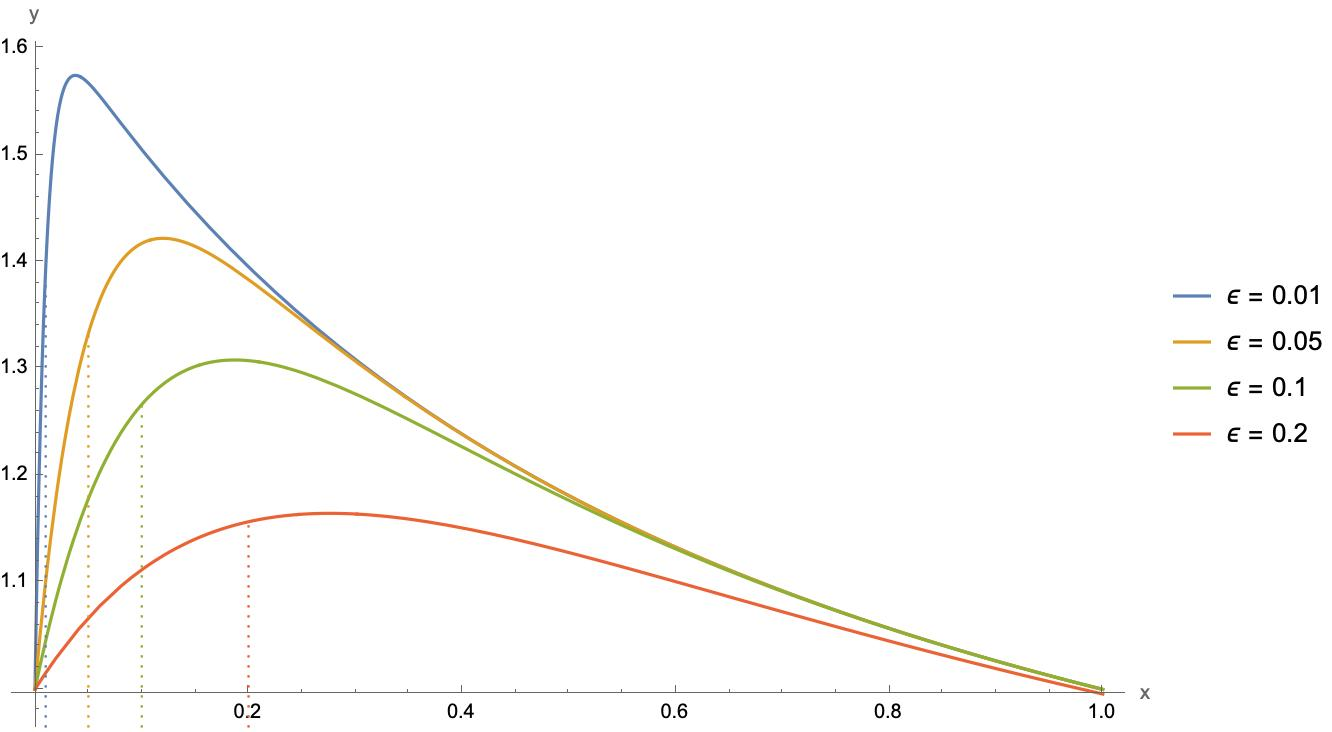
\includegraphics[width=14cm]{568_HW5_Plot1.jpg}
            \caption{Leading order uniform solution for different $\epsilon$ values. Boundary layer parameters $\delta(\epsilon)$ are shown as dotted lines.}
        \end{figure}


    \end{enumerate}

    \item Consider the singular equation:

    $$\epsilon y'' - x^2 y' - y = 0$$

    with $y(0)=y(1) =1$ and with $0 < \epsilon \ll 1$. 

    \begin{enumerate}
        \item With the method of dominant balance, show that there are three distinguished limits: $\delta = \epsilon^{1/2}$, $\delta = \epsilon$, and $\delta =1$ (the outer problem). Write down each of the problems in the various distinguished limits.

        \textbf{Solution:} We note that the coefficient of the first derivative term, $b(x)$, is positive definite for all $0<x \le 1$, and is $0$ at $x=0$. Hence, we expect a boundary layer at $x=0$ as well as $x=1$, as well as an "outer" region between the two boundary layers. 

        For the first boundary layer, near $x=0$, we define the stretched spacial coordinate $\xi = x/\delta$. Applying the chain rule, our transformed equation is 

        \begin{align*}
            \frac{\epsilon}{\delta^2} y_{\xi \xi} - \delta \xi^2 y_{\xi} - y = 0 && \Rightarrow && \epsilon y_{\xi \xi} - \delta^3 \xi^2 y_\xi - \delta^2 y = 0
        \end{align*}

        The dominant terms are $\epsilon y_{\xi \xi}$ and $\delta^2 y$. To balance the two terms, we need $\delta^2 \sim \epsilon$, hence, we let $\delta_l = \epsilon^{1/2}$. This is the asymptotic width of the left boundary layer. 

        For the second boundary layer, near $x=1$, we use the stretched coordinate $\xi = (1-x)/\delta$. Then our transformed equation becomes 

        \begin{align*}
            \frac{\epsilon}{\delta^2} y_{\xi\xi} + \frac{1}{\delta} (1- \delta \xi)^2 y_\xi - y = 0 && \Rightarrow && \epsilon y_{\xi\xi} + \delta (1-\delta \xi)^2 y_\xi - \delta^2 y = 0
        \end{align*}

        Here we find the dominant terms to be $\epsilon y_{\xi\xi}$ and $\delta y_\xi$. To balance these terms, we need $\epsilon \sim \delta$, and hence we let $\delta_r = \epsilon$ be the the asymptotic spacial scaling factor of the right boundary layer. 

        We find that are both left and right boundary layers, with $\delta = \epsilon^{1/2}$ and $\delta= \epsilon$, respectively. In addition, there is an "outer region" for which $\delta =1$. 

        \item Obtain the leading order uniform approximation. (Hint: there are boundary layers at $x=0$ and $x=1$).

        \textbf{Solution:} Since we have two boundary layers, we must solve in each region individually and apply the left and right boundary conditions, respectively. We begin with the left boundary layer.

        Near $x=0$ we have $\delta = \sqrt \epsilon$ and $\xi = x/\sqrt \epsilon$. Making the coordinate transformation to $\xi$ gives us

        \begin{align*}
            y_{\xi\xi} - \sqrt \epsilon \xi^2 y_\xi - y = 0
        \end{align*}

        and to leading order we have

        \begin{align*}
            y_{\xi\xi} - y = 0 && \Rightarrow &&  y_l(\xi) = B e^{\xi} + A e^{-\xi}
        \end{align*}

        For this solution to be bounded as $\xi\rightarrow \infty$, we need $B = 0$. To satisfy our left boundary condition we also require that $1=y_l(0) = A$. Hence we find the inner solution for the left boundary layer to be 

        $$y_l(x) = e^{-x/\sqrt{\epsilon}}$$

        For the second boundary layer solution near $x=1$ we have from part (a) that $\delta = \epsilon$, and $\xi = (1-x)/\epsilon$. Hence the governing equation is given by 

        \begin{align*}
            y_{\xi \xi} + y_\xi = 0 && \Rightarrow && y_r(\xi) = A e^{-\xi} +B
        \end{align*}

        To satisfy our right boundary condition we must have $1=y_r(1)=A+B \Rightarrow B = 1-A$, so we may write 
        
        $$y_r(\xi) = A e^{-\xi} + 1 - A$$

        Since $y_r$ is always bounded as $\xi \rightarrow \infty$, we retain the integration constant $A$, which we can use to satisfy our matching conditions.

        Lastly, we have the outer region $\delta \ll x \ll 1-\delta$, where we have $\delta =1$. In this regime, we have the governing equation

        \begin{align*}
            -x^2 y' -y = 0 && \Rightarrow && y_{out} = Ce^{1/x}
        \end{align*}

        To match this solution with the solution in the left boundary layer we must have 

        $$\lim_{\xi \rightarrow \infty} y_l(\xi) = \lim_{x \rightarrow 0} y_{out}$$

        Since $y_l \rightarrow 0$, we must have $C = 0$, and hence $y_{out} = 0$. Therefore, the matching condition for the right boundary layer solution is 

        $$\lim_{\xi \rightarrow \infty} y_r(\xi) = 0$$

        which means that $A=1$, and $y_r(x)=\exp((x-1)/\epsilon)$.

        We may now write our uniform solution as 

        \begin{align*}
            y_{unif} &= y_l + y_r + y_{out} -y_{match,l} - y_{match,r}\\
            &= e^{-x/\sqrt{\epsilon}} + e^{(x-1)/\epsilon}
        \end{align*}

        \item Plot the uniform solution for $\epsilon=0.01, 0.05, 0.1, 0.2$. 
        
        \textbf{Solution:} 

        \begin{figure}[H]
            \centering
            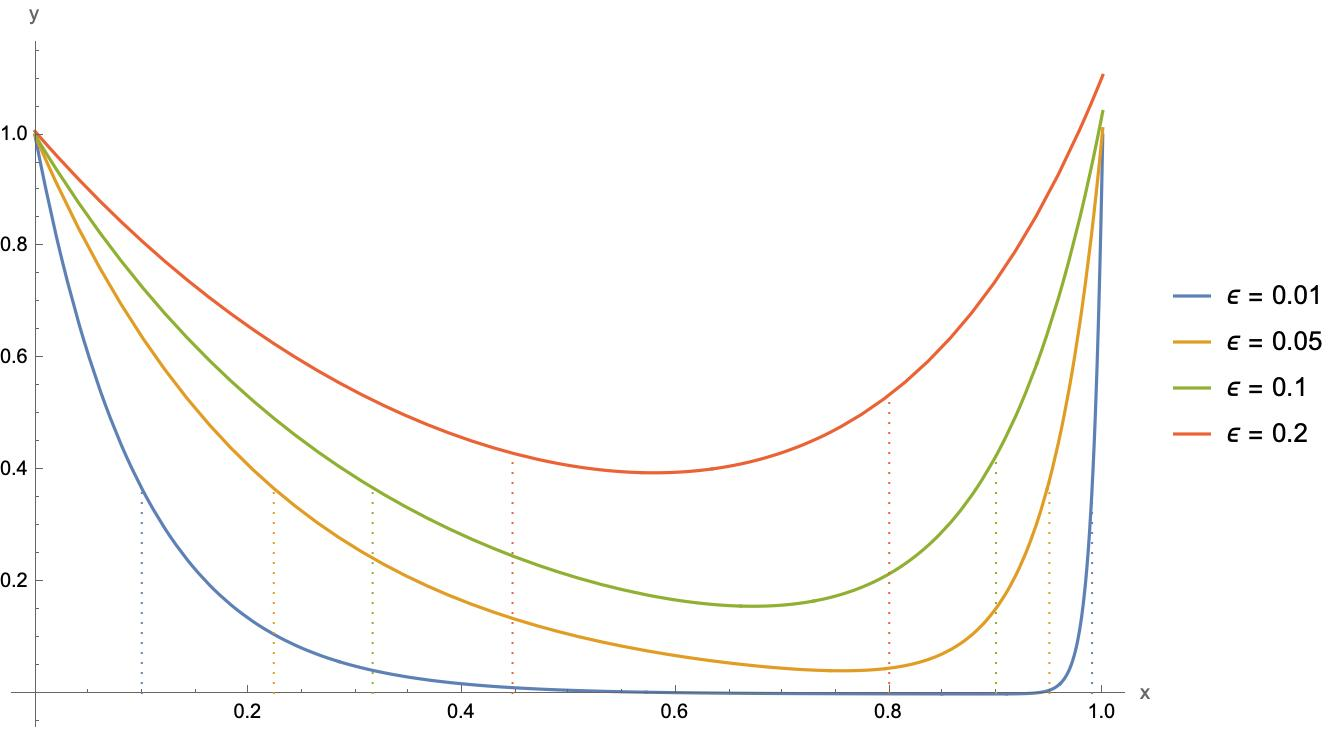
\includegraphics[width=14cm]{568_HW5_Plot2.jpg}
            \caption{Leading order uniform solution for different $\epsilon$ values. Boundary layer parameters $\delta_l(\epsilon)$ and $\delta_r(\epsilon)$ are shown as dotted lines.}
        \end{figure}
    \end{enumerate}
\end{enumerate}

\end{document}